% Options for packages loaded elsewhere
\PassOptionsToPackage{unicode}{hyperref}
\PassOptionsToPackage{hyphens}{url}
\PassOptionsToPackage{dvipsnames,svgnames,x11names}{xcolor}
%
\documentclass[
  12pt,
  letterpaper,
]{book}

\usepackage{amsmath,amssymb}
\usepackage{iftex}
\ifPDFTeX
  \usepackage[T1]{fontenc}
  \usepackage[utf8]{inputenc}
  \usepackage{textcomp} % provide euro and other symbols
\else % if luatex or xetex
  \usepackage{unicode-math}
  \defaultfontfeatures{Scale=MatchLowercase}
  \defaultfontfeatures[\rmfamily]{Ligatures=TeX,Scale=1}
\fi
\usepackage{lmodern}
\ifPDFTeX\else  
    % xetex/luatex font selection
\fi
% Use upquote if available, for straight quotes in verbatim environments
\IfFileExists{upquote.sty}{\usepackage{upquote}}{}
\IfFileExists{microtype.sty}{% use microtype if available
  \usepackage[]{microtype}
  \UseMicrotypeSet[protrusion]{basicmath} % disable protrusion for tt fonts
}{}
\makeatletter
\@ifundefined{KOMAClassName}{% if non-KOMA class
  \IfFileExists{parskip.sty}{%
    \usepackage{parskip}
  }{% else
    \setlength{\parindent}{0pt}
    \setlength{\parskip}{6pt plus 2pt minus 1pt}}
}{% if KOMA class
  \KOMAoptions{parskip=half}}
\makeatother
\usepackage{xcolor}
\usepackage[margin=1in]{geometry}
\setlength{\emergencystretch}{3em} % prevent overfull lines
\setcounter{secnumdepth}{5}
% Make \paragraph and \subparagraph free-standing
\makeatletter
\ifx\paragraph\undefined\else
  \let\oldparagraph\paragraph
  \renewcommand{\paragraph}{
    \@ifstar
      \xxxParagraphStar
      \xxxParagraphNoStar
  }
  \newcommand{\xxxParagraphStar}[1]{\oldparagraph*{#1}\mbox{}}
  \newcommand{\xxxParagraphNoStar}[1]{\oldparagraph{#1}\mbox{}}
\fi
\ifx\subparagraph\undefined\else
  \let\oldsubparagraph\subparagraph
  \renewcommand{\subparagraph}{
    \@ifstar
      \xxxSubParagraphStar
      \xxxSubParagraphNoStar
  }
  \newcommand{\xxxSubParagraphStar}[1]{\oldsubparagraph*{#1}\mbox{}}
  \newcommand{\xxxSubParagraphNoStar}[1]{\oldsubparagraph{#1}\mbox{}}
\fi
\makeatother

\usepackage{color}
\usepackage{fancyvrb}
\newcommand{\VerbBar}{|}
\newcommand{\VERB}{\Verb[commandchars=\\\{\}]}
\DefineVerbatimEnvironment{Highlighting}{Verbatim}{commandchars=\\\{\}}
% Add ',fontsize=\small' for more characters per line
\usepackage{framed}
\definecolor{shadecolor}{RGB}{241,243,245}
\newenvironment{Shaded}{\begin{snugshade}}{\end{snugshade}}
\newcommand{\AlertTok}[1]{\textcolor[rgb]{0.68,0.00,0.00}{#1}}
\newcommand{\AnnotationTok}[1]{\textcolor[rgb]{0.37,0.37,0.37}{#1}}
\newcommand{\AttributeTok}[1]{\textcolor[rgb]{0.40,0.45,0.13}{#1}}
\newcommand{\BaseNTok}[1]{\textcolor[rgb]{0.68,0.00,0.00}{#1}}
\newcommand{\BuiltInTok}[1]{\textcolor[rgb]{0.00,0.23,0.31}{#1}}
\newcommand{\CharTok}[1]{\textcolor[rgb]{0.13,0.47,0.30}{#1}}
\newcommand{\CommentTok}[1]{\textcolor[rgb]{0.37,0.37,0.37}{#1}}
\newcommand{\CommentVarTok}[1]{\textcolor[rgb]{0.37,0.37,0.37}{\textit{#1}}}
\newcommand{\ConstantTok}[1]{\textcolor[rgb]{0.56,0.35,0.01}{#1}}
\newcommand{\ControlFlowTok}[1]{\textcolor[rgb]{0.00,0.23,0.31}{\textbf{#1}}}
\newcommand{\DataTypeTok}[1]{\textcolor[rgb]{0.68,0.00,0.00}{#1}}
\newcommand{\DecValTok}[1]{\textcolor[rgb]{0.68,0.00,0.00}{#1}}
\newcommand{\DocumentationTok}[1]{\textcolor[rgb]{0.37,0.37,0.37}{\textit{#1}}}
\newcommand{\ErrorTok}[1]{\textcolor[rgb]{0.68,0.00,0.00}{#1}}
\newcommand{\ExtensionTok}[1]{\textcolor[rgb]{0.00,0.23,0.31}{#1}}
\newcommand{\FloatTok}[1]{\textcolor[rgb]{0.68,0.00,0.00}{#1}}
\newcommand{\FunctionTok}[1]{\textcolor[rgb]{0.28,0.35,0.67}{#1}}
\newcommand{\ImportTok}[1]{\textcolor[rgb]{0.00,0.46,0.62}{#1}}
\newcommand{\InformationTok}[1]{\textcolor[rgb]{0.37,0.37,0.37}{#1}}
\newcommand{\KeywordTok}[1]{\textcolor[rgb]{0.00,0.23,0.31}{\textbf{#1}}}
\newcommand{\NormalTok}[1]{\textcolor[rgb]{0.00,0.23,0.31}{#1}}
\newcommand{\OperatorTok}[1]{\textcolor[rgb]{0.37,0.37,0.37}{#1}}
\newcommand{\OtherTok}[1]{\textcolor[rgb]{0.00,0.23,0.31}{#1}}
\newcommand{\PreprocessorTok}[1]{\textcolor[rgb]{0.68,0.00,0.00}{#1}}
\newcommand{\RegionMarkerTok}[1]{\textcolor[rgb]{0.00,0.23,0.31}{#1}}
\newcommand{\SpecialCharTok}[1]{\textcolor[rgb]{0.37,0.37,0.37}{#1}}
\newcommand{\SpecialStringTok}[1]{\textcolor[rgb]{0.13,0.47,0.30}{#1}}
\newcommand{\StringTok}[1]{\textcolor[rgb]{0.13,0.47,0.30}{#1}}
\newcommand{\VariableTok}[1]{\textcolor[rgb]{0.07,0.07,0.07}{#1}}
\newcommand{\VerbatimStringTok}[1]{\textcolor[rgb]{0.13,0.47,0.30}{#1}}
\newcommand{\WarningTok}[1]{\textcolor[rgb]{0.37,0.37,0.37}{\textit{#1}}}

\providecommand{\tightlist}{%
  \setlength{\itemsep}{0pt}\setlength{\parskip}{0pt}}\usepackage{longtable,booktabs,array}
\usepackage{calc} % for calculating minipage widths
% Correct order of tables after \paragraph or \subparagraph
\usepackage{etoolbox}
\makeatletter
\patchcmd\longtable{\par}{\if@noskipsec\mbox{}\fi\par}{}{}
\makeatother
% Allow footnotes in longtable head/foot
\IfFileExists{footnotehyper.sty}{\usepackage{footnotehyper}}{\usepackage{footnote}}
\makesavenoteenv{longtable}
\usepackage{graphicx}
\makeatletter
\def\maxwidth{\ifdim\Gin@nat@width>\linewidth\linewidth\else\Gin@nat@width\fi}
\def\maxheight{\ifdim\Gin@nat@height>\textheight\textheight\else\Gin@nat@height\fi}
\makeatother
% Scale images if necessary, so that they will not overflow the page
% margins by default, and it is still possible to overwrite the defaults
% using explicit options in \includegraphics[width, height, ...]{}
\setkeys{Gin}{width=\maxwidth,height=\maxheight,keepaspectratio}
% Set default figure placement to htbp
\makeatletter
\def\fps@figure{htbp}
\makeatother
% definitions for citeproc citations
\NewDocumentCommand\citeproctext{}{}
\NewDocumentCommand\citeproc{mm}{%
  \begingroup\def\citeproctext{#2}\cite{#1}\endgroup}
\makeatletter
 % allow citations to break across lines
 \let\@cite@ofmt\@firstofone
 % avoid brackets around text for \cite:
 \def\@biblabel#1{}
 \def\@cite#1#2{{#1\if@tempswa , #2\fi}}
\makeatother
\newlength{\cslhangindent}
\setlength{\cslhangindent}{1.5em}
\newlength{\csllabelwidth}
\setlength{\csllabelwidth}{3em}
\newenvironment{CSLReferences}[2] % #1 hanging-indent, #2 entry-spacing
 {\begin{list}{}{%
  \setlength{\itemindent}{0pt}
  \setlength{\leftmargin}{0pt}
  \setlength{\parsep}{0pt}
  % turn on hanging indent if param 1 is 1
  \ifodd #1
   \setlength{\leftmargin}{\cslhangindent}
   \setlength{\itemindent}{-1\cslhangindent}
  \fi
  % set entry spacing
  \setlength{\itemsep}{#2\baselineskip}}}
 {\end{list}}
\usepackage{calc}
\newcommand{\CSLBlock}[1]{\hfill\break\parbox[t]{\linewidth}{\strut\ignorespaces#1\strut}}
\newcommand{\CSLLeftMargin}[1]{\parbox[t]{\csllabelwidth}{\strut#1\strut}}
\newcommand{\CSLRightInline}[1]{\parbox[t]{\linewidth - \csllabelwidth}{\strut#1\strut}}
\newcommand{\CSLIndent}[1]{\hspace{\cslhangindent}#1}

% header.tex
\usepackage{xcolor}        % Para colores
\usepackage{polyglossia}   % Soporte de idiomas con XeLaTeX
\setdefaultlanguage{spanish}

% Definición de colores personalizados
\definecolor{fecundidad}{HTML}{FFC125}      % Amarillo
\definecolor{supervivencia}{HTML}{36648B}   % Azul
\definecolor{crecimiento}{HTML}{548B54}     % Verde
\definecolor{retroceso}{HTML}{7A378B}       % Violeta
\definecolor{permanencia}{HTML}{26466A}     % Azul oscuro
\makeatletter
\@ifpackageloaded{caption}{}{\usepackage{caption}}
\AtBeginDocument{%
\ifdefined\contentsname
  \renewcommand*\contentsname{Table of contents}
\else
  \newcommand\contentsname{Table of contents}
\fi
\ifdefined\listfigurename
  \renewcommand*\listfigurename{List of Figures}
\else
  \newcommand\listfigurename{List of Figures}
\fi
\ifdefined\listtablename
  \renewcommand*\listtablename{List of Tables}
\else
  \newcommand\listtablename{List of Tables}
\fi
\ifdefined\figurename
  \renewcommand*\figurename{Figure}
\else
  \newcommand\figurename{Figure}
\fi
\ifdefined\tablename
  \renewcommand*\tablename{Table}
\else
  \newcommand\tablename{Table}
\fi
}
\@ifpackageloaded{float}{}{\usepackage{float}}
\floatstyle{ruled}
\@ifundefined{c@chapter}{\newfloat{codelisting}{h}{lop}}{\newfloat{codelisting}{h}{lop}[chapter]}
\floatname{codelisting}{Listing}
\newcommand*\listoflistings{\listof{codelisting}{List of Listings}}
\makeatother
\makeatletter
\makeatother
\makeatletter
\@ifpackageloaded{caption}{}{\usepackage{caption}}
\@ifpackageloaded{subcaption}{}{\usepackage{subcaption}}
\makeatother

\ifLuaTeX
  \usepackage{selnolig}  % disable illegal ligatures
\fi
\usepackage{bookmark}

\IfFileExists{xurl.sty}{\usepackage{xurl}}{} % add URL line breaks if available
\urlstyle{same} % disable monospaced font for URLs
\hypersetup{
  pdftitle={Diagnóstico poblacional: Introducción},
  colorlinks=true,
  linkcolor={Maroon},
  filecolor={Maroon},
  citecolor={Blue},
  urlcolor={Blue},
  pdfcreator={LaTeX via pandoc}}


\title{Diagnóstico poblacional: Introducción}
\author{}
\date{}

\begin{document}
\frontmatter
\maketitle

\renewcommand*\contentsname{Table of contents}
{
\hypersetup{linkcolor=}
\setcounter{tocdepth}{2}
\tableofcontents
}

\mainmatter
Por: Raymond L Tremblay, Ernesto Mujica, Demetria Mondragón

\subsection{Librerías de R requeridas para el siguiente
módulo}\label{libreruxedas-de-r-requeridas-para-el-siguiente-muxf3dulo}

\begin{Shaded}
\begin{Highlighting}[]
\FunctionTok{library}\NormalTok{(ggplot2)}
\end{Highlighting}
\end{Shaded}

\begin{center}\rule{0.5\linewidth}{0.5pt}\end{center}

\chapter{Objetivo y fundamentos de la conservación
biológica}\label{objetivo-y-fundamentos-de-la-conservaciuxf3n-bioluxf3gica}

El propósito central de la conservación biológica es garantizar la
persistencia de las especies, asegurando su supervivencia, reproducción
y la producción de descendencia viable a lo largo de generaciones. Este
objetivo requiere la consideración de factores intrínsecos y
extrínsecos, tanto bióticos como abióticos, y sus interacciones. No
obstante, la incorporación exhaustiva de todas las interacciones
posibles resulta impracticable. Por ello, es necesario simplificar el
problema mediante la identificación y priorización de los procesos más
determinantes. El desafío metodológico consiste en desarrollar modelos
que sean lo suficientemente parsimoniosos para facilitar su
interpretación, pero lo bastante complejos para capturar los mecanismos
esenciales de la dinámica poblacional.

\chapter{Importancia del hábitat en la
conservación}\label{importancia-del-huxe1bitat-en-la-conservaciuxf3n}

El primer requisito para la conservación efectiva es la disponibilidad y
protección de hábitats adecuados para cada especie. Durante las últimas
cinco décadas, se han observado cambios sustanciales en la cobertura y
manejo de ecosistemas en diversas regiones. Por ejemplo, en Puerto Rico,
la cobertura boscosa aumentó de aproximadamente 2--5 \% en la década de
1910 a más del 40 \% en el año 2000 (Parés-Ramos, Gould \& Aide, 2008;
Gould et al., 2017). De manera general, en América Latina se ha
registrado una tendencia hacia la reforestación en años recientes (Aide
et al., 2013), aunque esta dinámica varía significativamente entre
países, tipos de hábitat y periodos temporales. En este contexto, la
protección y restauración de hábitats constituye el primer principio
operativo para la conservación biológica.

La actividad antropogénica ha generado hábitats completamente nuevos,
resultado de la modificación de ecosistemas naturales, la introducción
de especies exóticas, la contaminación ambiental y el cambio climático.
Muchos de estos hábitats corresponden a bosques secundarios,
fragmentados y dominados por especies introducidas, lo que los hace
sustancialmente diferentes del ambiente original previo a las
transformaciones humanas. Como consecuencia, las especies de interés
suelen presentar una reducción significativa en el tamaño poblacional y
patrones de distribución altamente fragmentados. Surge entonces la
pregunta: ¿son suficientes estos remanentes poblacionales para mantener
la viabilidad de la especie? ¿Cómo se determina que una población es
viable?

Tradicionalmente, la conservación se ha fundamentado en la premisa de
que la protección del hábitat garantiza la persistencia de las especies.
No obstante, la mera presencia de individuos en un área protegida,
incluso en abundancia, no asegura su supervivencia a largo plazo. Un
ejemplo paradigmático es la extinción del Dodo (\emph{Raphus
cucullatus}), ave endémica de la isla de Mauricio, y su estrecha
relación funcional con \emph{Calvaria major}, una especie arbórea de la
familia Sapotaceae que estuvo al borde de la extinción. Aunque el último
Dodo fue registrado en 1681, Calvaria major persiste hasta la
actualidad. Stanley Temple (1977) demostró que el reclutamiento de esta
especie dependía del Dodo, dado que la germinación de sus semillas
requería el paso por el tracto digestivo de un ave para eliminar el
endocarpo persistente que inducía latencia (``dormancy'') (Temple,
1977). Este caso evidencia que la supervivencia futura de una especie no
puede asumirse sin considerar sus interacciones bióticas y abióticas.
Más de tres siglos después de la extinción del Dodo, \emph{Calvaria
major} sobrevive, aunque en un estado de alta vulnerabilidad.

\chapter{¿Qué es el estudio de la dinámica
poblacional?}\label{quuxe9-es-el-estudio-de-la-dinuxe1mica-poblacional}

La dinámica poblacional busca considerar todas las etapas y clases de
edad de las especies, así como sus interacciones, para evaluar cuáles
tienen un impacto relativamente mayor sobre la supervivencia de la
especie. Identificar estas etapas críticas permite determinar cuáles
podrían modificarse para influir en el crecimiento de las poblaciones
estudiadas, siempre considerando las interacciones con su entorno
biótico y abiótico.

La dinámica de poblaciones es fundamental en todas las áreas de la
ecología y la evolución. Comprenderla es clave para interpretar la
importancia relativa del acceso a los recursos y los efectos de la
competencia, la herbivoría y la depredación sobre la viabilidad de las
especies y la persistencia de las poblaciones. Tradicionalmente, los
estudios se enfocaban en el análisis de tablas de vida para el manejo,
la fenología y la conservación de especies particulares (Harper, 1977).
Sin duda, John L. Harper fue uno de los pioneros de la ecología vegetal
y dejó una amplia diversidad de publicaciones y temas (Sagar, 1985). En
años más recientes, los estudios se han diversificado para evaluar las
interacciones entre las especies y su ambiente (Caswell, 2001; Bacaër,
2011).

\chapter{Definición}\label{definiciuxf3n}

La definición más precisa de los estudios de dinámica poblacional se
refiere al análisis de los factores que influyen en el crecimiento, la
estabilidad y la reducción del tamaño de una población a lo largo del
tiempo. Por ejemplo, la dinámica poblacional de especies invasoras suele
incluir un periodo inicial de crecimiento muy lento durante la
colonización de un nuevo sitio, seguido por una fase de crecimiento
exponencial y, posteriormente, una disminución en la tasa de crecimiento
poblacional. La figura siguiente ilustra el cambio en el número de
individuos a lo largo del tiempo para una especie invasora hipotética.
Lo fundamental es que la dinámica poblacional constituye una herramienta
clave para evaluar el impacto de diferentes factores sobre el
crecimiento poblacional y su viabilidad.

\begin{Shaded}
\begin{Highlighting}[]
\FunctionTok{ggplot}\NormalTok{(pressure, }\FunctionTok{aes}\NormalTok{(temperature, pressure))}\SpecialCharTok{+}
  \FunctionTok{geom\_point}\NormalTok{()}\SpecialCharTok{+}
\NormalTok{  rlt\_theme}\SpecialCharTok{+}
  \FunctionTok{xlab}\NormalTok{(}\StringTok{"Tiempo"}\NormalTok{)}\SpecialCharTok{+}
  \FunctionTok{ylab}\NormalTok{(}\StringTok{"Tamaño poblacional, N"}\NormalTok{)}
\end{Highlighting}
\end{Shaded}

\begin{figure}[H]

{\centering 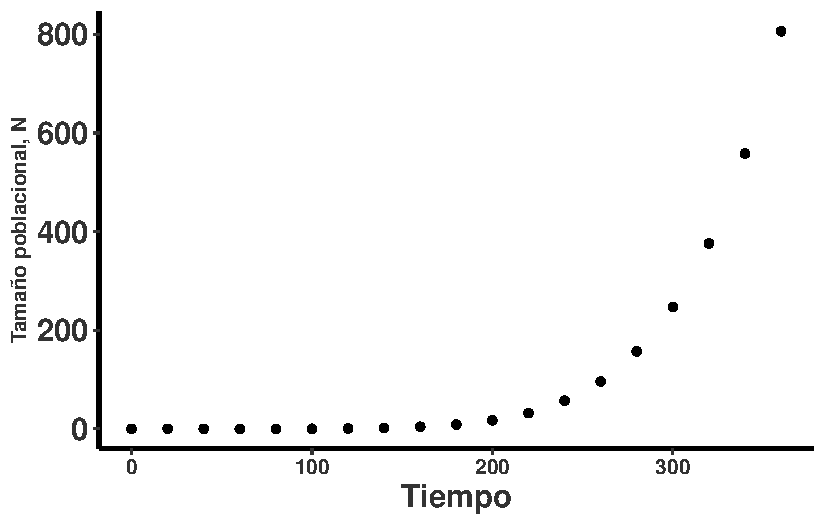
\includegraphics{102-Intro_files/figure-pdf/Pop-fig_1-1.pdf}

}

\caption{Cambio poblacional en tiempo}

\end{figure}%

\chapter{Un recuento histórico breve de la ecología de
poblaciones}\label{un-recuento-histuxf3rico-breve-de-la-ecologuxeda-de-poblaciones}

Los primeros estudios poblacionales se enfocaron en contar cuántos
individuos de varias especies había en un sitio y en evaluar el impacto
de diferentes tipos de efectos antropogénicos o de especies invasoras
(Crawley, 1990). Crawley (Crawley, 1990) indica que los primeros
estudios publicados sobre el conteo de individuos en plantas fueron
realizados por Carr (1848) y Burdon (1856), ambos presidentes de la
Tyneside Natural History Society en Inglaterra. En la publicación de
Burdon se menciona la presencia de individuos de \emph{Cypripedium
calceolus} en Castle Eden Dene, en el condado de Durham, hasta la
pérdida completa de todos los individuos en 1850 (extraído de la
revisión de Michael J. Crawley (Crawley, 1990)). Sin embargo, al evaluar
la publicación original, desafortunadamente no se menciona la cantidad
exacta de individuos en el sitio (Baker \& Tate, 1867).

Otro estudio pionero sobre dinámica poblacional fue establecido por V.
M. Spalding en 1906 en el Carnegie Institute Desert Laboratory, con el
objetivo de contabilizar la cantidad de individuos del cactus saguaro
(\emph{Carnegiea gigantea}) y evaluar la reducción de esta especie en
relación con el aumento de la especie invasora \emph{Prosopis
glandulosa} y su correlación con el incremento de la ganadería en el
área.

En su revisión sobre la dinámica de poblaciones de plantas, Crawley
(Crawley, 1990) identifica siete componentes consistentes en la biología
vegetal:

• Plasticidad del tamaño: El tamaño de las plantas es una característica
plástica, por lo que no constituye un buen indicador de la edad. Las
correlaciones entre tamaño y edad varían entre especies (Gatsuk et al.,
1980; Roux \& McGeoch, 2004; Vanderklein et al., 2007; Baden et al.,
2021).

• Interacciones con vecinos: Debido a que las plantas son organismos
sedentarios, la interacción con sus vecinos inmediatos es crucial. La
densidad de individuos circundantes afecta su crecimiento, reproducción
y supervivencia (Mitchell-Olds, 1987; Pantone, Baker \& Jordan, 1992;
Postma et al., 2021). En la revisión de Postma (Postma et al., 2021),
basada en 334 experimentos, se observa que al aumentar la densidad, el
tamaño de las plantas disminuye junto con el número de tallos y ramas,
aunque la altura permanece estable.

• Cambios sucesionales: Las variaciones en la estructura poblacional a
lo largo del tiempo son la norma, no la excepción (Young, Ewel \& Brown,
1987; Peña-Domene, Martı́nez-Garza \& Howe, 2013). Por ello, el
reclutamiento y la supervivencia en una parcela específica pueden variar
significativamente en tiempo y espacio, influenciados por factores
bióticos y abióticos (Acácio et al., 2007; Luzuriaga \& Escudero, 2008).

• Reclutamiento impredecible: El reclutamiento puede ser infrecuente,
impredecible y variable en el tiempo. Muchas especies forman bancos de
semillas, lo que permite que el reclutamiento provenga de semillas
almacenadas durante años (Saatkamp, Poschlod \& Venable, 2014; Fenner,
2017; Tomowski et al., 2023), incluso de diferentes cohortes.

• Competencia asimétrica: La competencia intraespecífica (Weiner \&
Thomas, 1986; Connolly \& Wayne, 1996; Weiner et al., 2001) e
interespecífica (Freckleton \& Watkinson, 2001) es común y generalmente
asimétrica: las plantas grandes afectan a las pequeñas, pero rara vez
ocurre lo contrario.

• Mortalidad relacionada al tamaño: La mortalidad está fuertemente
asociada al tamaño, siendo más frecuente en etapas o tamaños pequeños,
tanto entre especies (Moles \& Westoby, 2006) como a nivel
intraespecífico (Fricke, Tewksbury \& Rogers, 2019).

• Oportunidades tras la muerte de individuos grandes: La muerte de
plantas grandes y viejas, ya sea por accidentes, herbivoría o
enfermedades, puede generar espacios que faciliten el reclutamiento
(Wright et al., 2003).

\chapter{El análisis de Dinámica Poblacional y su
uso}\label{el-anuxe1lisis-de-dinuxe1mica-poblacional-y-su-uso}

Determinar el tamaño poblacional futuro tiene múltiples aplicaciones,
que pueden agruparse en tres grandes categorías: 1) comprender las
interacciones ecológicas, 2) manejo y conservación, y 3) procesos
evolutivos. Los estudios enfocados en conservación se enmarcan dentro
del enfoque de viabilidad poblacional.

En este libro presentaremos una introducción a cada una de estas
vertientes. Nuestros ejemplos son ilustrativos y no constituyen una
profundización exhaustiva de cada tema. En la siguiente tabla se
muestran algunos usos específicos de la metodología de matriz de
proyección poblacional (MPP). La lista de aplicaciones proviene en parte
de las ideas de Morris y Doak (Morris \& Doak, 2002), con ampliaciones
posteriores.

\section{Tabla: El uso potencial de la diferentes acercamiento de
PPM.}\label{tabla-el-uso-potencial-de-la-diferentes-acercamiento-de-ppm.}

\begin{longtable}[]{@{}
  >{\raggedright\arraybackslash}p{(\columnwidth - 6\tabcolsep) * \real{0.2500}}
  >{\raggedright\arraybackslash}p{(\columnwidth - 6\tabcolsep) * \real{0.2500}}
  >{\raggedright\arraybackslash}p{(\columnwidth - 6\tabcolsep) * \real{0.2500}}
  >{\raggedleft\arraybackslash}p{(\columnwidth - 6\tabcolsep) * \real{0.2500}}@{}}
\toprule\noalign{}
\begin{minipage}[b]{\linewidth}\raggedright
Categoría de Uso
\end{minipage} & \begin{minipage}[b]{\linewidth}\raggedright
Uso especifico
\end{minipage} & \begin{minipage}[b]{\linewidth}\raggedright
Referencias generales
\end{minipage} & \begin{minipage}[b]{\linewidth}\raggedleft
Referencias con Orquídeas
\end{minipage} \\
\midrule\noalign{}
\endhead
\bottomrule\noalign{}
\endlastfoot
Manejo & Identificar las etapas o procesos demográficos claves &
(Crouse, Crowder \& Caswell, 1987) & (Shefferson et al., 2003; Kéry \&
Gregg, 2004; Zotz \& Schmidt, 2006; Zhongjian et al., 2008; Tremblay et
al., 2009a,b) \\
& Determinar cuántos individuos en una población son necesarios para
reducir el riesgo de extinción & (Shaffer, 1981; Armbruster \& Lande,
1993; Traill, Bradshaw \& Brook, 2007; Flather et al., 2011) & \\
& Determinar cuántos individuos se necesitan introducir en un sitio para
establecer una población viable & (Bustamante, 1996; Bell, Bowles \&
McEachern, 2003) & \\
& Determinar cuántos individuos se pueden extraer sin afectar
negativamente la viabilidad de una población & (Nantel, Gagnon \& Nault,
1996; Ticktin et al., 2002; Ghimire et al., 2008; Jansen et al., 2018) &
(Ticktin et al., 2020; Emeterio-Lara et al., 2021) \\
& En especies invasoras, determinar cuántos individuos y en qué etapas
se deben remover para controlar la población & (Caplat, Coutts \&
Buckley, 2012; Arroyo-Cosultchi et al., 2022) & \\
& Determinar cuántas poblaciones se necesitan para lograr la viabilidad
de una especie a nivel local o global & (Lindenmayer \& Possingham,
1996) & (Tremblay, Meléndez-Ackerman \& Kapan, 2006; Lind et al., 2007;
Winkler, Hülber \& Hietz, 2009; Garcı́a, Goni \& Guzmán, 2010; Kindlmann,
Meléndez-Ackerman \& Tremblay, 2014) \\
Evaluación de riesgos & Evaluar el riesgo de extinción de una población
& (Gotelli \& Ellison, 2006) & (Nicolè, Brzosko \& Till-Bottraud, 2005;
Iriondo Alegria et al., 2009; Hutchings, 2010; Thorpe et al., 2011;
Raventós et al., 2015; Hens et al., 2017; Ackerman et al., 2020; Berry
\& Cleavitt, 2021; Timsina et al., 2021) \\
& Comparar el riesgo relativo entre dos o más poblaciones o especies &
(Earl, 2019) & (Schödelbauerová, Tremblay \& Kindlmann, 2010; Raventós
et al., 2018; Crain, Tremblay \& Ferguson, 2019) \\
Interacciones ecológicas & Evaluar interacciones ecológicas abióticas y
bióticas para entender las variables importantes para la supervivencia
de una población & (Halpern \& Underwood, 2006; Mandle, Ticktin \&
Zuidema, 2015; Ehrlen et al., 2016; Souza, Schmidt \& Conceicao, 2018) &
(Coates, Lunt \& Tremblay, 2006; Sletvold, Øien \& Moen, 2010; Sletvold
et al., 2013; Ospina-Calderón et al., 2023) \\
Procesos y patrones evolutivos & Identificar procesos, interacciones y
patrones evolutivos del ciclo de vida que impactan el crecimiento
poblacional & (Coste \& Pavard, 2020) & (Calvo, 1993; Jäkäläniemi et
al., 2011; Shefferson et al., 2012; Falcón, Ackerman \& Tremblay,
2017) \\
Metodología & Identificar la metodología adecuada según el tipo de
muestreo o historia de vida & (Van Groenendael et al., 1994; Gerlach Jr
\& Rice, 2003; Rademaker, Leeuwen \& Smallegange, 2024; Jops, Dalling \&
O'Dwyer, 2025) & (Kéry \& Gregg, 2004; Gregg \& Kéry, 2006; Tremblay et
al., 2009b, 2021; Shefferson, Warren \& Pulliam, 2014; Tremblay \&
McCarthy, 2014) \\
\end{longtable}

\chapter{Usos de la dinámica
poblacional}\label{usos-de-la-dinuxe1mica-poblacional}

\section{Identificar las etapas o procesos demográficos
claves}\label{identificar-las-etapas-o-procesos-demogruxe1ficos-claves}

Es fundamental reconocer cuáles son las etapas de vida más susceptibles
a cambios bióticos y abióticos, así como su impacto sobre la
persistencia de una población. Un ejemplo clásico en la literatura,
utilizando modelos matriciales por etapas (PPM), son los estudios sobre
la dinámica poblacional de la tortuga boba o cabezona (\emph{Caretta
caretta}) (Crouse, Crowder \& Caswell, 1987; Crowder et al., 1994).
Crouse y Crowder demostraron que, aun salvando todos los huevos de la
depredación, esta estrategia tendría un impacto mínimo en el crecimiento
poblacional. El mayor efecto sobre la tasa de crecimiento se lograría
protegiendo a los adultos, específicamente reduciendo su mortalidad en
redes de pesca mediante modificaciones que permitan su escape sin
ahogarse. Estos trabajos fueron pioneros en mostrar que es posible
simular diferentes escenarios basados en la historia de vida del
organismo y evaluar su impacto. Esto no implica que no se deba proteger
los huevos, sino que el beneficio es menor comparado con la protección
de los adultos.

En estudios realizados en Cuba hace casi 20 años sobre tres especies
epífitas (\emph{Cattleyopsis cubensis}, \emph{Dendrophylax lindenii} y
\emph{Encyclia bocourtii}), se demostró que la protección de individuos
adultos es esencial para mantener el equilibrio poblacional. Esto se
debe al alto valor reproductivo de los individuos más grandes, que
poseen mayor capacidad para reemplazar a los individuos jóvenes, los
cuales presentan mayor probabilidad de morir (Raventós et al., 2021).
Entre los principales riesgos para estas especies se encuentran la
incidencia de huracanes, la mortalidad de las especies que actúan como
forófitos y, en menor medida, la depredación.

\section{Determinar cuántos individuos en una población son necesarios
para reducir el riesgo de
extinción}\label{determinar-cuuxe1ntos-individuos-en-una-poblaciuxf3n-son-necesarios-para-reducir-el-riesgo-de-extinciuxf3n}

El efecto del tamaño poblacional sobre la biología y la probabilidad de
extinción en poblaciones naturales está bien documentado (Shaffer \&
Samson, 1985; Nunney \& Campbell, 1993; Harris et al., 2022). Surge
entonces la pregunta: ¿cuál es la probabilidad de extinción de una
población considerando la cantidad de individuos en cada etapa del ciclo
de vida?

En general, se observa que a menor tamaño poblacional (N), mayor es el
riesgo de extinción. Sin embargo, esta correlación puede variar si
algunas etapas del ciclo de vida presentan reducciones significativas o
si la probabilidad de sobrevivir o avanzar a la siguiente etapa es muy
baja.

En el caso de las orquídeas, se sabe que una de las etapas más
vulnerables es la de semilla, ya que en condiciones naturales depende
del establecimiento de una interacción micorrícica específica. Por
ejemplo, ¿cuál es la probabilidad de que las semillas se depositen en un
sitio adecuado, encuentren su hongo específico, germinen y cuenten con
las condiciones ambientales necesarias para crecer hasta convertirse en
juveniles? Estas transiciones son extremadamente raras.

Por consiguiente, al evaluar la viabilidad de una nueva población de
orquídeas, no basta con considerar la cantidad de individuos presentes;
también es necesario estimar la probabilidad de que las semillas lleguen
a convertirse en adultos reproductores. Darwin (Darwin, 1877) estimó que
un fruto de \emph{Orchis maculata} produce aproximadamente 6,200
semillas, y una planta puede generar hasta 30 cápsulas, lo que equivale
a 186,300 semillas. En un acre, la suma de todas las plantas podría
producir más de 32,400,000,000 semillas. Sin duda, la probabilidad de
que una semilla germine y llegue a ser una planta adulta es
extremadamente baja; de lo contrario, estaríamos cubiertos de orquídeas
en apenas dos generaciones.

\section{Determinar cuántos individuos se necesita introducir en un
sitio para establecer una población
viable}\label{determinar-cuuxe1ntos-individuos-se-necesita-introducir-en-un-sitio-para-establecer-una-poblaciuxf3n-viable}

Determinar cuántos individuos se necesitan introducir en un sitio para
establecer una población viable es una pregunta clave en conservación.
Naturalmente, a mayor cantidad de individuos reintroducidos, mayor será
la probabilidad de éxito, asumiendo que el área seleccionada permite la
supervivencia, crecimiento y reproducción en todas las etapas del ciclo
de vida. Sin embargo, los recursos son limitados, por lo que la pregunta
debería enfocarse en cuál es el número mínimo de individuos necesario
para garantizar un porcentaje determinado de éxito en el establecimiento
de una nueva población.

En los últimos años, diversas organizaciones y científicos han
implementado programas de reintroducción de especies en sus hábitats
nativos, e incluso en áreas urbanas (Bellis et al., 2024; D'Agostino et
al., 2024).

En Corea, dos estudios ilustran la complejidad del proceso. En la isla
de Jeju, se translocó la orquídea Thrixspermum japonicum, cuya población
original era de aproximadamente 50 individuos, de los cuales solo uno
produjo frutos. A partir de este individuo se propagaron plántulas que
fueron reintroducidas en el sitio. De los 216 individuos translocados,
el 73\% sobrevivió el primer año y el 63\% el segundo año; entre el 16\%
y el 35\% produjo frutos en los dos años siguientes (Kim, Kang \& Kim,
2016). En otro estudio, en la isla de Bogildo, se reintrodujeron más de
13,000 individuos de Dendrobium moniliforme propagados artificialmente.
Los autores demostraron que la ubicación y las condiciones del
microhábitat son variables críticas: las áreas abiertas con luz solar
directa favorecieron un crecimiento más rápido que las zonas sombreadas,
y la especie de árbol huésped también influyó significativamente (Kim,
Kang \& Kim, 2016).

Desafortunadamente, ninguno de estos estudios aplicó métodos de análisis
de viabilidad poblacional (PVA) para determinar el tamaño mínimo de
reintroducción necesario para establecer poblaciones viables. Además, no
se consideraron factores como la probabilidad de germinación y el éxito
en alcanzar la etapa adulta. Un ejemplo de esta complejidad es el
trabajo de Zoe Fae Smith (Smith, 2006), quien evaluó la germinación in
situ de \emph{Diuris fragrantissima} y \emph{D. punctata} en Australia
utilizando 640 mallas según el método de (Rasmussen \& Whigham, 1993).
Ninguna semilla germinó en campo, lo que evidencia la necesidad de
estudios más detallados sobre viabilidad y estrategias de
reintroducción.

En otro estudio, Zettler y colaboradores (Zettler \& McInnis, 1993)
evaluaron la germinación de semillas de \emph{Goodyera pubescens} en un
sitio de reintroducción en el estado de Illinois, EE.UU. Los autores
encontraron que la germinación de las semillas fue muy baja y que la
presencia de hongos micorrícicos específicos era esencial para este
proceso. En consecuencia, la reintroducción de orquídeas en un sitio
debe considerar la presencia de hongos micorrícicos adecuados, así como
la cantidad de individuos que se deberían reintroducir para garantizar
la viabilidad de la población.

\section{Determinación del número de individuos que pueden ser extraídos
sin comprometer la viabilidad
poblacional}\label{determinaciuxf3n-del-nuxfamero-de-individuos-que-pueden-ser-extrauxeddos-sin-comprometer-la-viabilidad-poblacional}

La extracción de individuos, seudobulbos o flores desde su ambiente
natural responde principalmente a tres propósitos:

\begin{itemize}
\tightlist
\item
  Obtención de individuos para programas de conservación ex situ.
\item
  Utilización de un grupo de individuos para su propagación.
\item
  Extracción con fines comerciales sin objetivos de conservación (por
  ejemplo, uso medicinal, cultivo ornamental u otros usos).
\end{itemize}

Se suele asumir que la colecta de individuos de especies de orquídeas
desde sus hábitats naturales, tanto para conservación ex situ como para
propagación comercial, tiene un impacto mínimo y no afecta la
supervivencia poblacional a largo plazo. Sin embargo, este supuesto
requiere una evaluación crítica. La historia del fanatismo por la
recolección de orquídeas con fines comerciales está bien documentada
(Subedi et al., 2013). Aunque se podría pensar que estas prácticas son
cosa del pasado, persisten casos de extracción ilegal por personas
inescrupulosas que no consideran el impacto sobre la población o la
especie (Hinsley et al., 2018).

Por lo tanto, la pregunta central es: ¿cuántos individuos, y en qué
etapas del ciclo de vida, pueden ser extraídos sin afectar negativamente
el crecimiento poblacional? (Ticktin et al., 2020). Responder esta
cuestión implica comprender la dinámica poblacional y aplicar modelos
que permitan estimar umbrales de extracción sostenible.

\section{En especies invasivas, determinar cuántos individuos y en qué
etapas se necesitan remover para controlar la
población.}\label{en-especies-invasivas-determinar-cuuxe1ntos-individuos-y-en-quuxe9-etapas-se-necesitan-remover-para-controlar-la-poblaciuxf3n.}

Actualmente, se reconoce ampliamente el impacto negativo que los
organismos invasores pueden ejercer sobre la flora y fauna nativas. Esto
plantea interrogantes fundamentales: ¿cuáles son las características que
confieren a una especie su potencial invasivo? y ¿qué programas de
manejo pueden implementarse para mitigar su impacto?

En términos generales, las especies invasoras se caracterizan por
presentar altas tasas de crecimiento y reproducción, elevada
supervivencia, baja mortalidad y gran capacidad de dispersión. Por
consiguiente, cualquier estrategia de manejo debe identificar las etapas
del ciclo de vida más vulnerables a la intervención. En la mayoría de
los casos, la etapa de semillas constituye el punto más susceptible para
la manipulación y control.

Los impactos más notorios de especies invasoras han sido documentados en
Australia, incluyendo la introducción del conejo (\emph{Oryctolagus
cuniculus}) (Alves et al., 2022) y del cactus \emph{Opuntia} (Novoa et
al., 2015), entre otros ejemplos ampliamente discutidos en cursos de
ecología de comunidades. No obstante, la problemática de las especies
invasoras continúa siendo un tema que requiere investigaciones y
evaluaciones más profundas.

Diversos estudios han empleado modelos de proyección poblacional (PPM)
para analizar la demografía de especies invasoras (Buckley, Briese \&
Rees, 2003; Koop \& Horvitz, 2005; McMahon \& Metcalf, 2008; Ramula et
al., 2008; Li \& Ramula, 2015). Un caso particular evaluó el efecto de
una hormiga invasora y un insecto nativo sobre la dinámica poblacional
de una orquídea invasora (Falcón, Ackerman \& Tremblay, 2017).

\section{Evaluar el riesgo de una
población}\label{evaluar-el-riesgo-de-una-poblaciuxf3n}

La mayoría de los estudios que emplean modelos de proyección poblacional
(PPM, por sus siglas en inglés) se centran en evaluar el riesgo de
reducción poblacional o de extinción. Un ejemplo clásico es el trabajo
de Forsman (Forsman et al., 1996), quien analizó 11 poblaciones del búho
moteado (spotted owl) y demostró que 10 de ellas estaban en declive,
mientras que la población de California se encontraba en riesgo de
extinción.

Los análisis basados en PPM como herramienta para estimar el riesgo de
extinción incluyen diferentes métricas, tales como la probabilidad de
extinción, la cuasiextinción y la probabilidad de cuasiextinción. Estas
estimaciones son fundamentales para especies cuyo manejo demográfico
busca reducir el riesgo de desaparición (Crone et al., 2011; Semmens et
al., 2016). Sin embargo, aunque este enfoque es común en la literatura
de conservación, puede resultar problemático si no se considera la
confiabilidad de los parámetros estimados y la incertidumbre asociada a
los datos (Ludwig, 1999).

Un ejemplo del uso de PPM en orquídeas amenazadas es el caso de
\emph{Crepidium acuminatum}, una especie en peligro de extinción del
sudeste asiático, afectada por la extracción para uso medicinal (Timsina
et al., 2021). Un estudio demográfico de seis años reveló que la tasa de
crecimiento poblacional fluctuó entre 0.80 y 1.05, sin diferencias
significativas entre años ni entre poblaciones. Otros ejemplos incluyen
el trabajo de (Borrero et al., 2023), quienes estudiaron
\emph{Trichocentrum undulatum} y evaluaron el riesgo asociado a su
ubicación en la periferia de la distribución. En ambos casos, el
objetivo fue estimar el riesgo de extinción de las poblaciones
analizadas.

\section{Determinación del número de poblaciones necesarias para la
viabilidad de una especie a nivel local o
global}\label{determinaciuxf3n-del-nuxfamero-de-poblaciones-necesarias-para-la-viabilidad-de-una-especie-a-nivel-local-o-global}

La mayoría de las especies están divididas en múltiples poblaciones,
aunque el concepto de ``población'' puede variar según el contexto. Con
frecuencia, los autores no explicitan la definición utilizada y emplean
el término para referirse simplemente a una agrupación de individuos. La
definición práctica más común considera una población como un conjunto
de individuos suficientemente cercanos entre sí, lo que facilita la
recolección de datos. Sin embargo, este enfoque puede carecer de validez
ecológica o evolutiva.

En ecología, una población debería definirse como un grupo de individuos
que interactúan entre sí, o que al menos tienen cierta probabilidad de
hacerlo. Por ejemplo, si hablamos de una población de \emph{Catasetum},
los individuos deberían estar lo suficientemente próximos para que las
abejas polinizadoras (i.e., \emph{Euglossa} spp.) puedan transportar el
polen entre ellos. La distancia y el potencial de movimiento de estas
abejas varían considerablemente según la especie y la estructura del
paisaje (Tonhasca, Albuquerque \& Blackmer, 2003; Pokorny et al., 2015;
Opedal et al., 2017).

Otra definición, de carácter evolutivo, considera una población como el
conjunto de individuos entre los cuales ocurre flujo génico a lo largo
de una generación. El tiempo generacional depende de la longevidad de la
especie, que puede variar ampliamente. Por ejemplo, en las orquídeas
epífitas de ramitas (twig epiphytes), el ciclo generacional puede ser de
3 a 4 años, mientras que en \emph{Cypripedium calceolus}, una especie
terrestre de zonas templadas, los individuos adultos pueden vivir más de
50 años. Cabe destacar que la ``longevidad'' se define como la mediana
de la edad de los individuos en una población, excluyendo casos
extremos. El único estudio que ha evaluado la longevidad en orquídeas es
(Tremblay, 2000), limitado a especies del género \emph{Lepanthes}.

\section{Cuál de los procesos y patrones evolutivos del ciclo de vida de
especies impacta su crecimiento o grupos
taxonómicos}\label{cuuxe1l-de-los-procesos-y-patrones-evolutivos-del-ciclo-de-vida-de-especies-impacta-su-crecimiento-o-grupos-taxonuxf3micos}

Un trabajo que aprovecha la MPP para evaluar procesos evolutivos es el
de Ricardo Calvo {[}@calvo1993evolutionary{]}, quien analizó la dinámica
poblacional de \emph{Tolumnia variegata} para determinar si la
limitación de polinizadores afecta su viabilidad. El estudio combinó
experimentos de polinización manual con modelos matriciales para estimar
la tasa de crecimiento poblacional bajo distintos niveles de
polinización. Los resultados mostraron que la fructificación natural es
extremadamente baja (\textless1 \%), pero aumenta significativamente con
polinización artificial, aunque con costos reproductivos en crecimiento
y floración futura. Las simulaciones sugieren que incluso una baja
producción de plántulas por fruto podría compensar estos costos,
favoreciendo la selección hacia mayor polinización. Sin embargo, la
persistencia de baja fructificación en orquídeas engañosas indica que la
estrategia puede ser estable si el reclutamiento de plántulas es
limitado, resaltando la importancia de considerar interacciones
ecológicas y datos de establecimiento para evaluar la viabilidad
poblacional. Este caso nos recuerda que la conservación y la evolución
no dependen solo de la presencia de individuos, sino de la compleja red
de procesos que sostienen la vida a largo plazo.

\begin{figure}[H]

{\centering 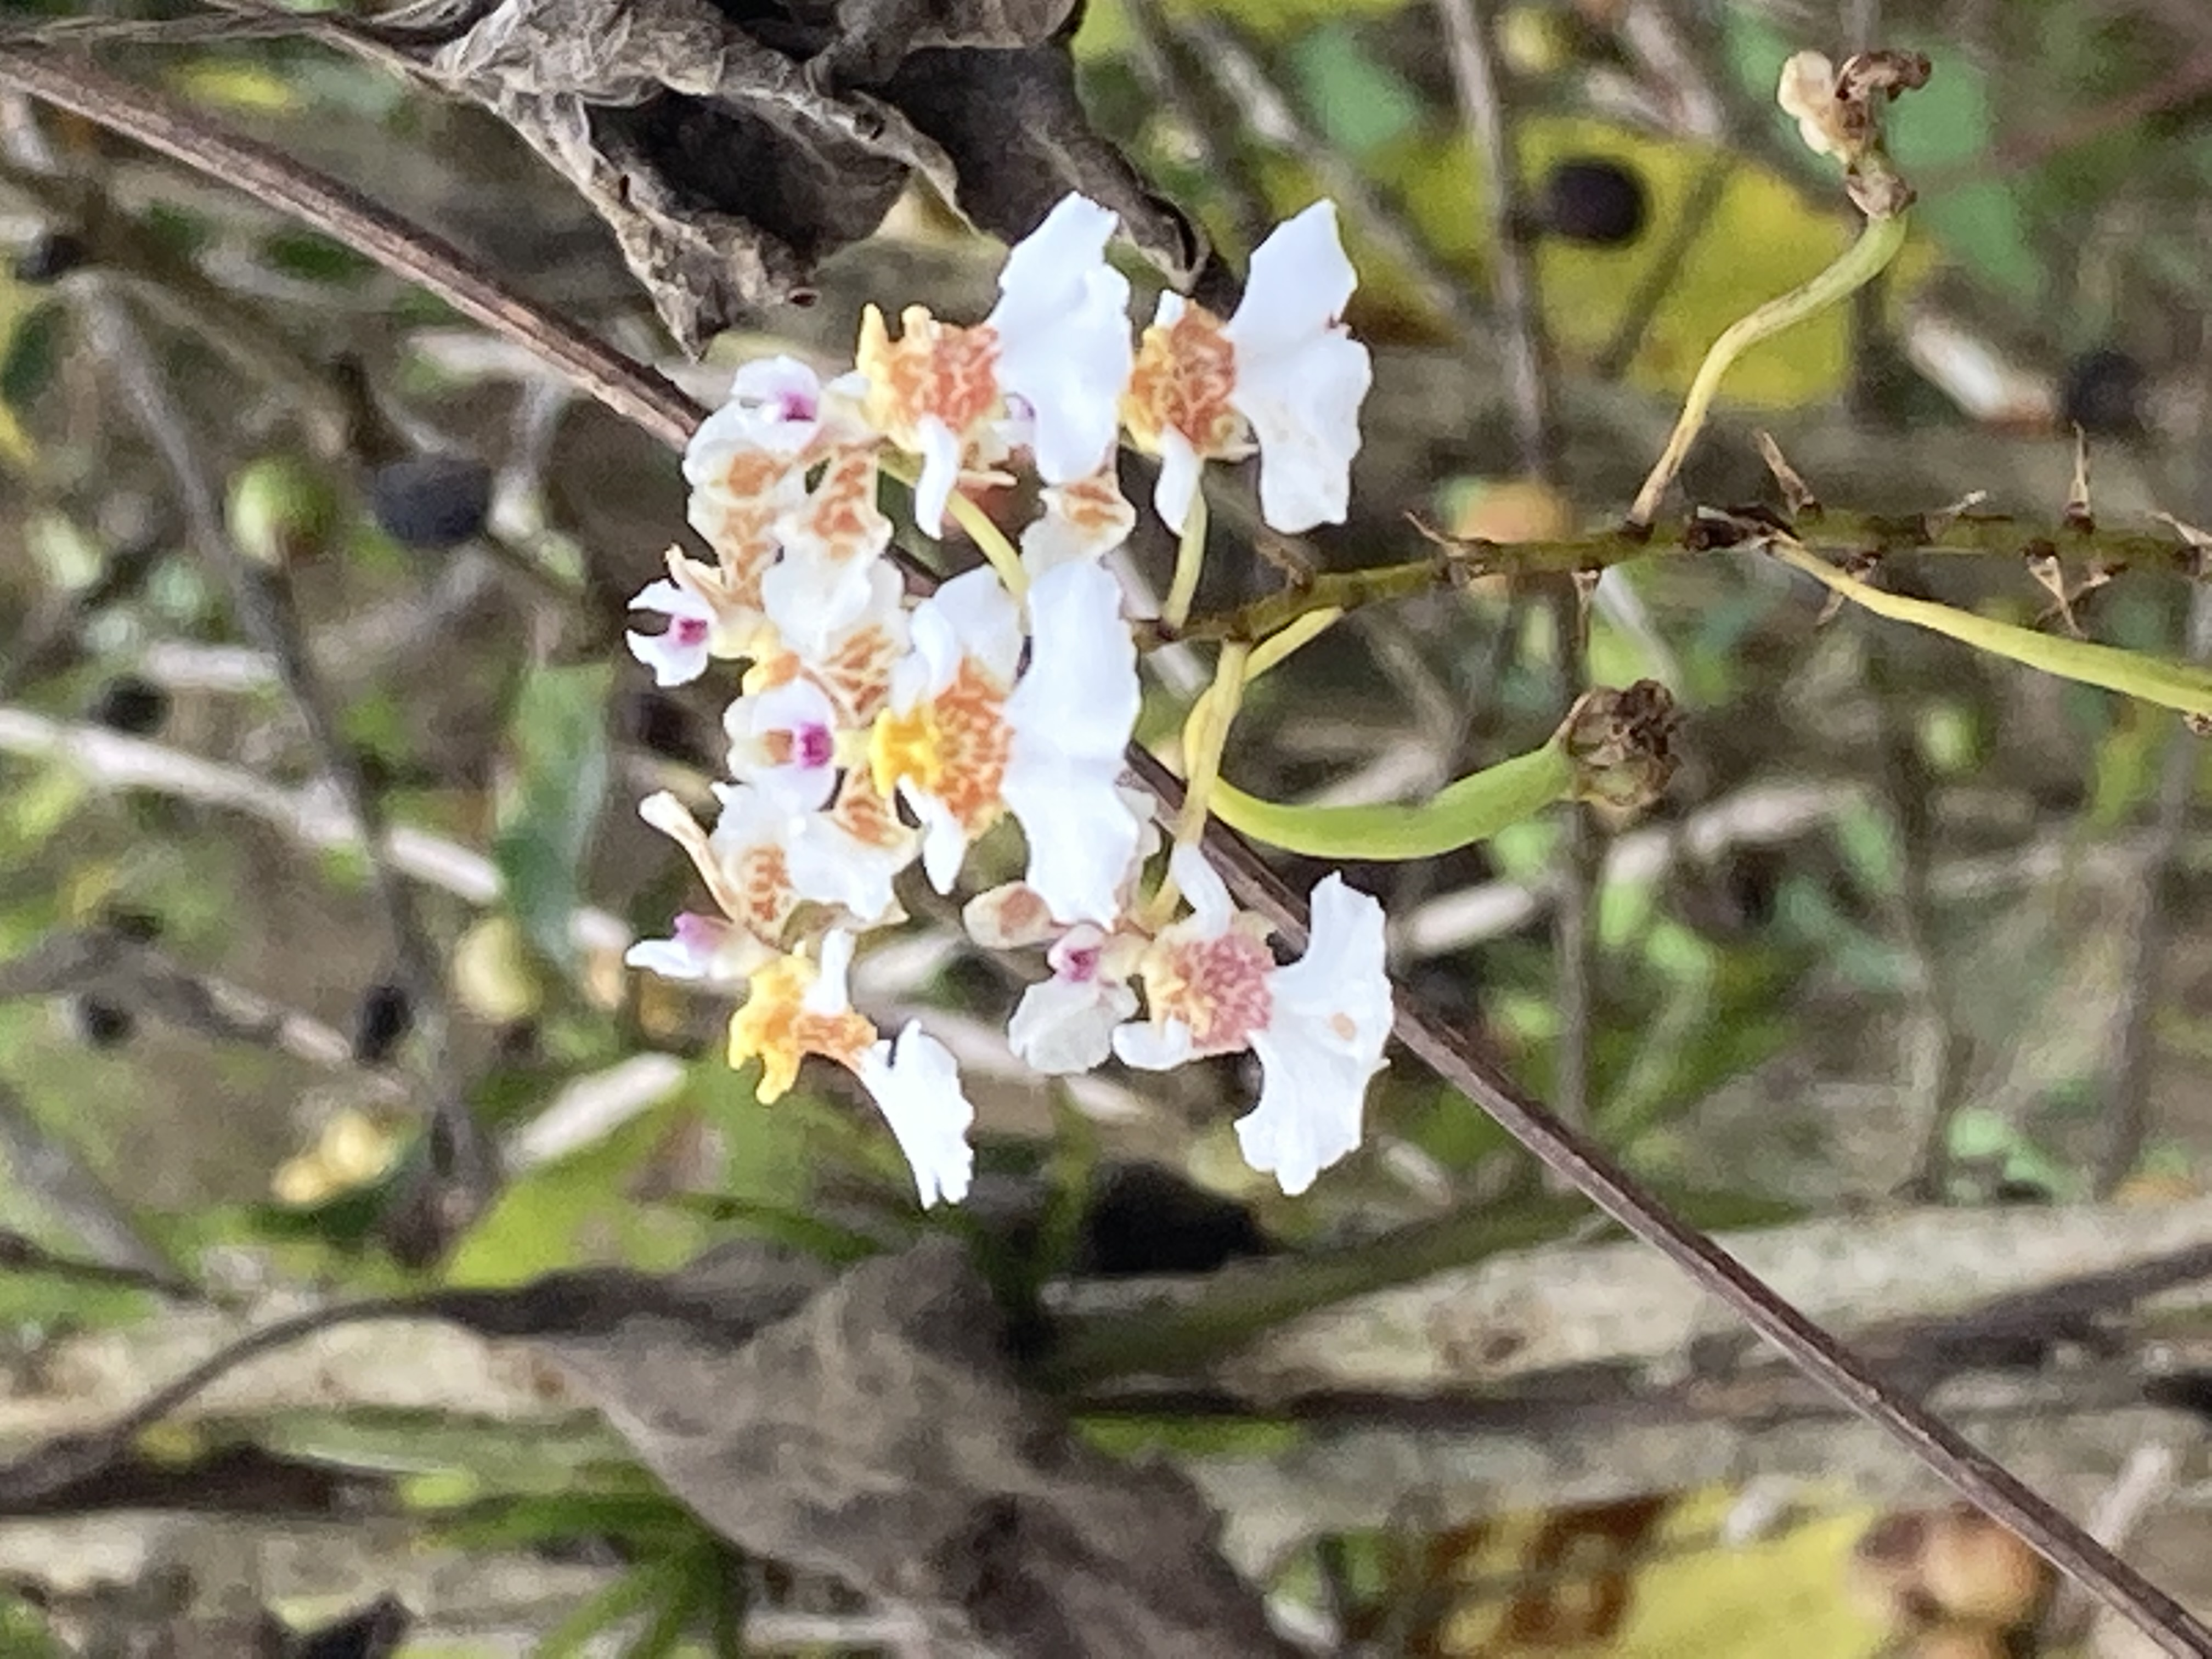
\includegraphics{Species/Tolumnia variegata Tremblay.jpeg}

}

\caption{\emph{Tolumnia variegata}. Foto: Tremblay}

\end{figure}%

\begin{center}\rule{0.5\linewidth}{0.5pt}\end{center}

\chapter{Visualización de la dinámica
poblacional}\label{visualizaciuxf3n-de-la-dinuxe1mica-poblacional}

Representar el cambio poblacional mediante diagramas y sus posibles
causas permite integrar los diferentes componentes bióticos y abióticos
que influyen en la dinámica de una especie. Es importante aclarar que un
modelo es una simplificación ---una ``caricatura''--- y no incluye todos
los factores que afectan la población. El objetivo de un modelo es
reducir la complejidad biológica a los procesos más relevantes; si se
complica en exceso, los patrones y dinámicas no pueden atribuirse a
efectos proporcionalmente importantes. Además, un modelo demasiado
específico sería aplicable solo a una especie o población, limitando su
utilidad en otros sistemas.

En la figura se ilustran los factores principales que influyen en el
crecimiento poblacional y las variables más relevantes para evaluar el
riesgo de extinción. Todo análisis de dinámica poblacional parte del
tamaño de la población (N) o su densidad, ya que este parámetro impacta
directamente otros factores demográficos. En el diagrama, las líneas
entrecortadas con signos de interrogación indican relaciones con poca o
nula evidencia en orquídeas, mientras que las líneas continuas
representan factores respaldados por estudios.

Los efectos denso-dependientes pueden influir en el número de individuos
en el siguiente intervalo, así como las diferencias genéticas entre
ellos. Aunque esto se ha documentado en otros organismos, en orquídeas
los estudios son escasos y suelen asumir que las diferencias genéticas
tienen mayor impacto. Por el contrario, los efectos estocásticos
---tanto demográficos como ambientales--- son bien conocidos en
orquídeas y afectan los parámetros de crecimiento y su variación.
Finalmente, la variación temporal es el factor que más incide en el
riesgo de extinción: cuando esta variación es alta en poblaciones
pequeñas, la probabilidad de extinción aumenta significativamente. Por
ello, la variación en el tiempo debe considerarse en todos los estudios
de dinámica poblacional.

\begin{center}\rule{0.5\linewidth}{0.5pt}\end{center}

\begin{figure}[H]

{\centering 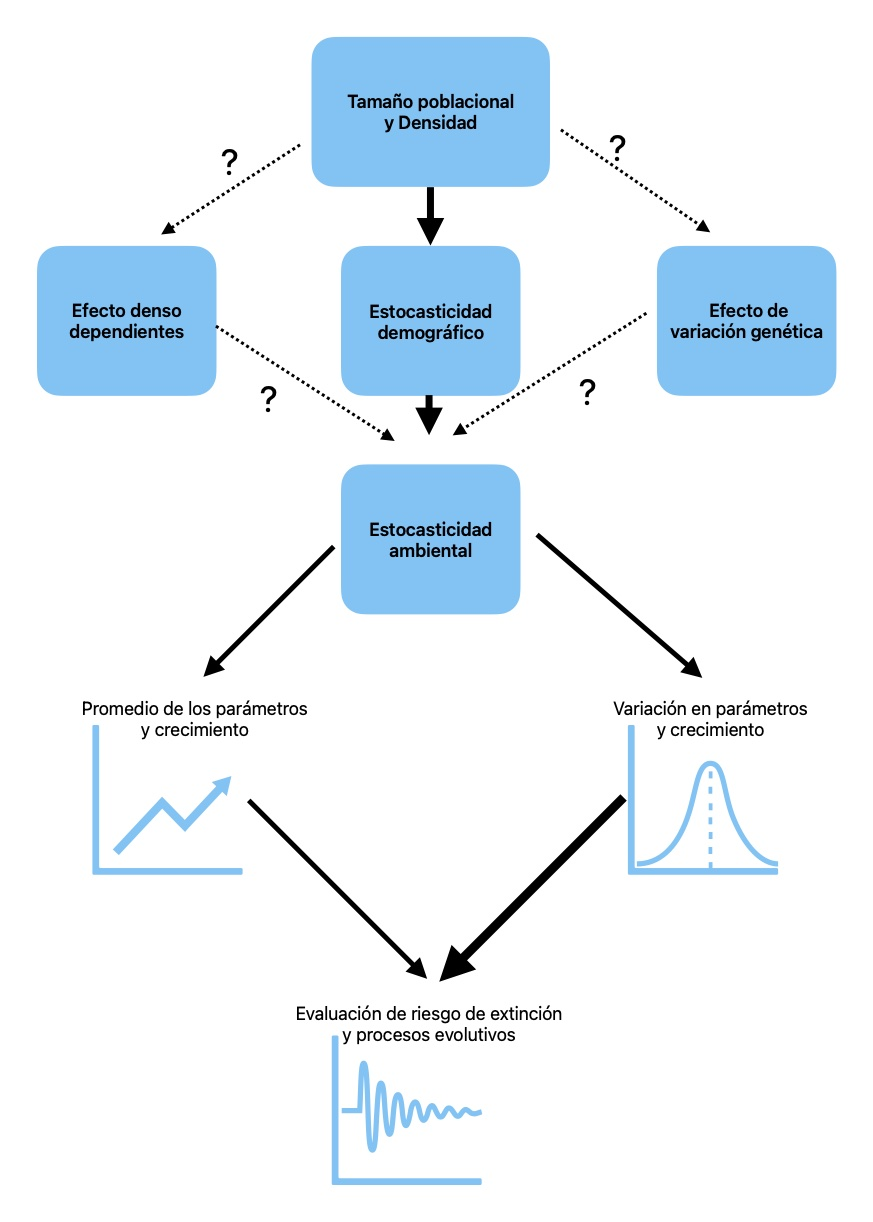
\includegraphics[width=0.5\textwidth,height=\textheight]{Figures/Demografia_de_una_poblacion.jpg}

}

\caption{Factores que influencia la dinámica de una población}

\end{figure}%

\begin{center}\rule{0.5\linewidth}{0.5pt}\end{center}

Revisión:

Sept 14, 2024

RLT Feb 11, 2025;

Ernesto Feb 13, 2025;

RLT Feb 18, 2025;

Tupac Feb 18, 2025

\phantomsection\label{refs}
\begin{CSLReferences}{1}{0}
\bibitem[\citeproctext]{ref-acacio2007multiple}
Acácio V, Holmgren M, Jansen PA, Schrotter O. 2007. Multiple recruitment
limitation causes arrested succession in mediterranean cork oak systems.
\emph{Ecosystems} 10:1220--1230.

\bibitem[\citeproctext]{ref-ackerman2020small}
Ackerman J, Tremblay R, Pérez M, Madden H, Bechtold M, Boeken M. 2020.
Small populations on small islands: What chance does an orchid have?
\emph{International Journal of Plant Sciences} 181:667--685.

\bibitem[\citeproctext]{ref-aide2013deforestation}
Aide TM, Clark ML, Grau HR, López-Carr D, Levy MA, Redo D,
Bonilla-Moheno M, Riner G, Andrade-Núñez MJ, Muñiz M. 2013.
Deforestation and reforestation of latin america and the caribbean
(2001--2010). \emph{Biotropica} 45:262--271.

\bibitem[\citeproctext]{ref-alves2022single}
Alves JM, Carneiro M, Day JP, Welch JJ, Duckworth JA, Cox TE, Letnic M,
Strive T, Ferrand N, Jiggins FM. 2022. A single introduction of wild
rabbits triggered the biological invasion of australia.
\emph{Proceedings of the National Academy of Sciences} 119:e2122734119.

\bibitem[\citeproctext]{ref-armbruster1993population}
Armbruster P, Lande R. 1993. A population viability analysis for african
elephant (\emph{loxodonta {a}fricana}): How big should reserves be?
\emph{Conservation Biology} 7:602--610.

\bibitem[\citeproctext]{ref-arroyo2022prescriptions}
Arroyo-Cosultchi G, Golubov J, Solórzano JV, Mandujano MC. 2022.
Prescriptions for the control of a clonal invasive species using
demographic models. \emph{Plants} 11:689.

\bibitem[\citeproctext]{ref-bacaer2011short}
Bacaër N. 2011. \emph{A {S}hort {H}istory of {M}athematical {P}opulation
{D}ynamics}. Springer.

\bibitem[\citeproctext]{ref-baden2021effects}
Baden HM, Roach D, Schweingruber FH, Reitzel K, Lundgreen K, Dahlgren
JP. 2021. The effects of age on the demography of a perennial plant
depend on interactions with size and environment. \emph{Journal of
Ecology} 109:1068--1077.

\bibitem[\citeproctext]{ref-baker1867northumberland}
Baker JD, Tate GR. 1867. \emph{A new flora of {N}orthumberland and
{D}urham}. Tyneside Naturalists' Field Club, London.

\bibitem[\citeproctext]{ref-bell2003projecting}
Bell T, Bowles M, McEachern A. 2003. Projecting the success of plant
population restoration with viability analysis. In: \emph{Population
viability in plants: Conservation, management, and modeling of rare
plants}. Springer, 313--348.

\bibitem[\citeproctext]{ref-bellis2024identifying}
Bellis J, Osazuwa-Peters O, Maschinski J, Keir MJ, Parsons EW, Kaye TN,
Kunz M, Possley J, Menges E, Smith SA, others. 2024. Identifying
predictors of translocation success in rare plant species.
\emph{Conservation Biology} 38:e14190.

\bibitem[\citeproctext]{ref-berry2021population}
Berry EJ, Cleavitt NL. 2021. Population dynamics and comparative
demographics in sympatric populations of the round-leaved orchids
\emph{{P}latanthera {m}acrophylla} and \emph{{P}. {o}rbiculata}.
\emph{Population Ecology} 63:274--289.

\bibitem[\citeproctext]{ref-borrero2023populations}
Borrero H, Oviedo-Prieto R, Alvarez JC, Ticktin T, Cisneros M, Liu H.
2023. Populations of a tropical epiphytic orchid are destabilized in its
peripheral range by hurricane and an exotic herbivore. \emph{Ecosphere}
14:e4355.

\bibitem[\citeproctext]{ref-buckley2003demography}
Buckley YM, Briese DT, Rees M. 2003. Demography and management of the
invasive plant species hypericum perforatum. II. Construction and use of
an individual-based model to predict population dynamics and the effects
of management strategies. \emph{Journal of Applied Ecology} 40:494--507.

\bibitem[\citeproctext]{ref-bustamante1996population}
Bustamante J. 1996. Population viability analysis of captive and
released bearded vulture populations. \emph{Conservation Biology}
10:822--831.

\bibitem[\citeproctext]{ref-calvo1993evolutionary}
Calvo RN. 1993. Evolutionary demography of orchids: Intensity and
frequency of pollination and the cost of fruiting. \emph{Ecology}
74:1033--1042. DOI:
\href{https://doi.org/10.2307/1940473}{10.2307/1940473}.

\bibitem[\citeproctext]{ref-caplat2012modeling}
Caplat P, Coutts S, Buckley YM. 2012. Modeling population dynamics,
landscape structure, and management decisions for controlling the spread
of invasive plants. \emph{Annals of the New York Academy of Sciences}
1249:72--83.

\bibitem[\citeproctext]{ref-caswell2001matrix}
Caswell H. 2001. \emph{Matrix {P}opulation {M}odels: Construction,
analysis, and interpretation}. Sunderland, Massachusetts, USA: Sinauer
Associates.

\bibitem[\citeproctext]{ref-coates2006effects}
Coates F, Lunt ID, Tremblay R. 2006. Effects of disturbance on
population dynamics of the threatened orchid \emph{{P}rasophyllum
{c}orrectum} DL jones and implications for grassland management in
south-eastern {A}ustralia. \emph{Biological Conservation} 129:59--69.

\bibitem[\citeproctext]{ref-connolly1996asymmetric}
Connolly J, Wayne P. 1996. Asymmetric competition between plant species.
\emph{Oecologia} 108:311--320.

\bibitem[\citeproctext]{ref-coste2020analysis}
Coste CF, Pavard S. 2020. Analysis of a multitrait population projection
matrix reveals the evolutionary and demographic effects of a life
history trade-off. \emph{Ecological Modelling} 418:108915.

\bibitem[\citeproctext]{ref-crain2019sheltered}
Crain B, Tremblay R, Ferguson J. 2019. Sheltered from the storm?
Population viability analysis of a rare endemic under periodic
catastrophe regimes. \emph{Population Ecology} 61:74--92. DOI:
\href{https://doi.org/10.1002/1438-390X.1002}{10.1002/1438-390X.1002}.

\bibitem[\citeproctext]{ref-crawley1990population}
Crawley MJ. 1990. The population dynamics of plants. \emph{Philosophical
Transactions of the Royal Society of London. Series B: Biological
Sciences} 330:125--140.

\bibitem[\citeproctext]{ref-crone2011plant}
Crone EE, Menges ES, Ellis MM, Bell T, Bierzychudek P, Ehrlén J, Kaye
TN, Knight TM, Lesica P, Morris WF, others. 2011. How do plant
ecologists use matrix population models? \emph{Ecology Letters} 14:1--8.

\bibitem[\citeproctext]{ref-crouse1987stage}
Crouse DT, Crowder LB, Caswell H. 1987. A stage-based population model
for loggerhead sea turtles and implications for conservation.
\emph{Ecology} 68:1412--1423.

\bibitem[\citeproctext]{ref-crowder1994predicting}
Crowder LB, Crouse DT, Heppell SS, Martin TH. 1994. Predicting the
impact of turtle excluder devices on loggerhead sea turtle populations.
\emph{Ecological Applications} 4:437--445.

\bibitem[\citeproctext]{ref-d2024best}
D'Agostino M, Cao Pinna L, Carboni M, Assini S, Bacchetta G, Bartolucci
F, Brancaleoni L, Buldrini F, Carta A, Cerabolini B, others. 2024. Best
practices, errors, and perspectives of half a century of plant
translocation in italy. \emph{Conservation Biology} 38:e14233.

\bibitem[\citeproctext]{ref-darwin1877various}
Darwin C. 1877. \emph{The various contrivances by which orchids are
fertilised by insects}. John Murray.

\bibitem[\citeproctext]{ref-earl2019evaluating}
Earl JE. 2019. Evaluating the assumptions of population projection
models used for conservation. \emph{Biological Conservation}
237:145--154.

\bibitem[\citeproctext]{ref-ehrlen2016advancing}
Ehrlen J, Morris WF, Euler T von, Dahlgren JP. 2016. Advancing
environmentally explicit structured population models of plants.
\emph{Journal of Ecology} 104:292--305.

\bibitem[\citeproctext]{ref-emeterio2021does}
Emeterio-Lara A, Garcı́a-Franco JG, Hernández-Apolinar M,
Toledo-Hernández VH, Valencia-Dı́az S, Flores-Palacios A. 2021. Does
extraction of orchids affect their population structure? Evidence from
populations of \emph{{L}aelia {a}utumnalis} ({O}rchidaceae).
\emph{Forest Ecology and Management} 480:118667.

\bibitem[\citeproctext]{ref-falcon2017quantifying}
Falcón W, Ackerman JD, Tremblay R. 2017. Quantifying how acquired
interactions with native and invasive insects influence population
growth rates of a non-indigenous plant. \emph{Biological Invasions}
19:895--911. DOI:
\href{https://doi.org/10.1007/s10530-016-1318-8}{10.1007/s10530-016-1318-8}.

\bibitem[\citeproctext]{ref-fenner2017ecology}
Fenner M. 2017. Ecology of seed banks. In: \emph{Seed development and
germination}. Routledge, 507--528.

\bibitem[\citeproctext]{ref-flather2011minimum}
Flather CH, Hayward GD, Beissinger SR, Stephens PA. 2011. Minimum viable
populations: Is there a `magic number'for conservation practitioners?
\emph{Trends in Ecology \& Evolution} 26:307--316.

\bibitem[\citeproctext]{ref-forsman1996demography}
Forsman E, Sovern S, Seaman DE, Maurice K, Taylor M, Zisa J. 1996.
Demography of the northern spotted owl on the olympic peninsula and east
slope of the cascade range, washington. \emph{Studies in Avian Biology}
17:21--30.

\bibitem[\citeproctext]{ref-freckleton2001asymmetric}
Freckleton R, Watkinson A. 2001. Asymmetric competition between plant
species. \emph{Functional Ecology} 15:615--623.

\bibitem[\citeproctext]{ref-fricke2019linking}
Fricke EC, Tewksbury JJ, Rogers HS. 2019. Linking intra-specific trait
variation and plant function: Seed size mediates performance tradeoffs
within species. \emph{Oikos} 128:1716--1725.

\bibitem[\citeproctext]{ref-garcia2010living}
Garcı́a MB, Goni D, Guzmán D. 2010. Living at the edge: Local versus
positional factors in the long-term population dynamics of an endangered
orchid. \emph{Conservation Biology} 24:1219--1229.

\bibitem[\citeproctext]{ref-gatsuk1980age}
Gatsuk L, Smirnova O, Vorontzova L, Zaugolnova L, Zhukova L. 1980. Age
states of plants of various growth forms: A review. \emph{The Journal of
Ecology}:675--696.

\bibitem[\citeproctext]{ref-gerlach2003testing}
Gerlach Jr JD, Rice KJ. 2003. Testing life history correlates of
invasiveness using congeneric plant species. \emph{Ecological
Applications} 13:167--179.

\bibitem[\citeproctext]{ref-ghimire2008demographic}
Ghimire SK, Gimenez O, Pradel R, McKey D, Aumeeruddy-Thomas Y. 2008.
Demographic variation and population viability in a threatened himalayan
medicinal and aromatic herb \emph{{N}ardostachys grandiflora}: Matrix
modelling of harvesting effects in two contrasting habitats.
\emph{Journal of Applied Ecology} 45:41--51.

\bibitem[\citeproctext]{ref-gotelli2006forecasting}
Gotelli NJ, Ellison AM. 2006. Forecasting extinction risk with
nonstationary matrix models. \emph{Ecological Applications} 16:51--61.

\bibitem[\citeproctext]{ref-gould2017land}
Gould WA, Wadsworth FH, Quiñones M, Fain SJ, Álvarez-Berrı́os NL. 2017.
Land use, conservation, forestry, and agriculture in {P}uerto {R}ico.
\emph{Forests} 8:242.

\bibitem[\citeproctext]{ref-gregg2006comparison}
Gregg KB, Kéry M. 2006. Comparison of size vs. Life-state classification
in demographic models for the terrestrial orchid \emph{{C}leistes
{b}ifaria}. \emph{Biological Conservation} 129:50--58.

\bibitem[\citeproctext]{ref-halpern2006approaches}
Halpern SL, Underwood N. 2006. Approaches for testing herbivore effects
on plant population dynamics. \emph{Journal of Applied Ecology}
43:922--929.

\bibitem[\citeproctext]{ref-harper1977population}
Harper JL. 1977. \emph{Population {B}iology of {P}lants}. Academic
Press.

\bibitem[\citeproctext]{ref-harris2022abundance}
Harris GM, Butler MJ, Stewart DR, Cain III JW. 2022. The abundance and
persistence of caprinae populations. \emph{Scientific Reports} 12:13807.

\bibitem[\citeproctext]{ref-hens2017low}
Hens H, Pakanen V-M, Jäkäläniemi A, Tuomi J, Kvist L. 2017. Low
population viability in small endangered orchid populations: Genetic
variation, seedling recruitment and stochasticity. \emph{Biological
Conservation} 210:174--183.

\bibitem[\citeproctext]{ref-hinsley2018review}
Hinsley A, De Boer HJ, Fay MF, Gale SW, Gardiner LM, Gunasekara RS,
Kumar P, Masters S, Metusala D, Roberts DL, others. 2018. A review of
the trade in orchids and its implications for conservation.
\emph{Botanical Journal of the Linnean Society} 186:435--455.

\bibitem[\citeproctext]{ref-hutchings2010population}
Hutchings M. 2010. The population biology of the early spider orchid
\emph{{O}phrys {s}phegodes} {M}ill. III. Demography over three decades.
\emph{Journal of Ecology} 98:867--878.

\bibitem[\citeproctext]{ref-iriondo2009peligro}
Iriondo Alegria J, Albert Gamboa M, Gimenez Benavides L, Dominguez
Lozano F, Escudero Alcantara A. 2009. \emph{Poblaciones en peligro:
Viabilidad demogr{á}fica de la flora vascular amenazada de espana}.
Direcci{ó}n General de Medio Ambiente y Pol{í}tica Forestal.

\bibitem[\citeproctext]{ref-jakalaniemi2011orchids}
Jäkäläniemi A, Crone EE, Närhi P, Tuomi J. 2011. Orchids do not pay
costs at emergence for prolonged dormancy. \emph{Ecology} 92:1538--1543.

\bibitem[\citeproctext]{ref-jansen2018towards}
Jansen M, Anten NP, Bongers F, Martı́nez-Ramos M, Zuidema PA. 2018.
Towards smarter harvesting from natural palm populations by sparing the
individuals that contribute most to population growth or productivity.
\emph{Journal of Applied Ecology} 55:1682--1691.

\bibitem[\citeproctext]{ref-jops2025life}
Jops K, Dalling JW, O'Dwyer JP. 2025. Life history is a key driver of
temporal fluctuations in tropical tree abundances. \emph{Proceedings of
the National Academy of Sciences} 122:e2422348122.

\bibitem[\citeproctext]{ref-kery2004demographic}
Kéry M, Gregg KB. 2004. Demographic analysis of dormancy and survival in
the terrestrial orchid \emph{{C}ypripedium {r}eginae}. \emph{Journal of
Ecology} 92:686--695.

\bibitem[\citeproctext]{ref-kim2016restoration}
Kim Y, Kang K-W, Kim K-J. 2016. Restoration of endangered orchid
species, \emph{{D}endrobium {m}oniliforme} (l.) sw.({O}rchidaceae) in
{K}orea. \emph{Korean Journal of Plant Taxonomy} 46:256--266.

\bibitem[\citeproctext]{ref-kindlmann2014disobedient}
Kindlmann P, Meléndez-Ackerman EJ, Tremblay R. 2014. Disobedient
epiphytes: Colonization and extinction rates in a metapopulation of
\emph{{L}epanthes {r}upestris} ({O}rchidaceae) contradict theoretical
predictions based on patch connectivity. \emph{Botanical Journal of the
Linnean Society} 175:598--606.

\bibitem[\citeproctext]{ref-koop2005projection}
Koop AL, Horvitz CC. 2005. Projection matrix analysis of the demography
of an invasive, nonnative shrub (\emph{{A}rdisia {e}lliptica}).
\emph{Ecology} 86:2661--2672.

\bibitem[\citeproctext]{ref-lindenmayer1996ranking}
Lindenmayer DB, Possingham HP. 1996. Ranking conservation and timber
management options for leadbeater's possum in southeastern australia
using population viability analysis. \emph{Conservation Biology}
10:235--251.

\bibitem[\citeproctext]{ref-lind2007metapopulation}
Lind H, Franzén M, Pettersson B, Anders Nilsson L. 2007. Metapopulation
pollination in the deceptive orchid \emph{{A}nacamptis {p}yramidalis}.
\emph{Nordic Journal of Botany} 25:176--182.

\bibitem[\citeproctext]{ref-li2015demographic}
Li S-L, Ramula S. 2015. Demographic strategies of plant invaders in
temporally varying environments. \emph{Population ecology} 57:373--380.

\bibitem[\citeproctext]{ref-ludwig1999meaningful}
Ludwig D. 1999. Is it meaningful to estimate a probability of
extinction? \emph{Ecology} 80:298--310.

\bibitem[\citeproctext]{ref-luzuriaga2008determines}
Luzuriaga AL, Escudero A. 2008. What determines emergence and net
recruitment in an early succession plant community? Disentangling biotic
and abiotic effects. \emph{Journal of Vegetation Science} 19:445--456.

\bibitem[\citeproctext]{ref-mandle2015resilience}
Mandle L, Ticktin T, Zuidema PA. 2015. Resilience of palm populations to
disturbance is determined by interactive effects of fire, herbivory and
harvest. \emph{Journal of Ecology} 103:1032--1043.

\bibitem[\citeproctext]{ref-mcmahon2008transient}
McMahon SM, Metcalf C. 2008. Transient sensitivities of non-indigenous
shrub species indicate complicated invasion dynamics. \emph{Biological
Invasions} 10:833--846.

\bibitem[\citeproctext]{ref-mitchell1987analysis}
Mitchell-Olds T. 1987. Analysis of local variation in plant size.
\emph{Ecology} 68:82--87.

\bibitem[\citeproctext]{ref-moles2006seed}
Moles AT, Westoby M. 2006. Seed size and plant strategy across the whole
life cycle. \emph{Oikos} 113:91--105.

\bibitem[\citeproctext]{ref-morris2002quantitative}
Morris WF, Doak DF. 2002. \emph{Quantitative conservation biology:
Theory and practice of population viability analysis}. Sinauer
Associates, Inc. Publishers.

\bibitem[\citeproctext]{ref-nantel1996population}
Nantel P, Gagnon D, Nault A. 1996. Population viability analysis of
american ginseng and wild leek harvested in stochastic environments.
\emph{Conservation Biology} 10:608--621.

\bibitem[\citeproctext]{ref-nicole2005population}
Nicolè F, Brzosko E, Till-Bottraud I. 2005. Population viability
analysis of \emph{{C}ypripedium {c}alceolus} in a protected area:
Longevity, stability and persistence. \emph{Journal of Ecology}
93:716--726.

\bibitem[\citeproctext]{ref-novoa2015introduced}
Novoa A, Le Roux JJ, Robertson MP, Wilson JR, Richardson DM. 2015.
Introduced and invasive cactus species: A global review. \emph{AoB
Plants} 7:plu078.

\bibitem[\citeproctext]{ref-nunney1993assessing}
Nunney L, Campbell KA. 1993. Assessing minimum viable population size:
Demography meets population genetics. \emph{Trends in {E}cology \&
{E}volution} 8:234--239.

\bibitem[\citeproctext]{ref-opedal2017euglossine}
Opedal ØH, Falahati-Anbaran M, Albertsen E, Armbruster WS,
Pérez-Barrales R, Stenøien HK, Pélabon C. 2017. Euglossine bees mediate
only limited long-distance gene flow in a tropical vine. \emph{New
Phytologist} 213:1898--1908.

\bibitem[\citeproctext]{ref-ospina2023effect}
Ospina-Calderón N, Tremblay R, Torres A, Flanagan N. 2023. The effect of
habitat transformation on a twig epiphytic orchid: Evidence from
population dynamics. \emph{Frontiers in Ecology and Evolution}
11:1135316.

\bibitem[\citeproctext]{ref-pantone1992path}
Pantone D, Baker J, Jordan P. 1992. Path analysis of red rice
(\emph{{O}ryza sativa} {L}.) competition by cultivated rice. \emph{Weed
Science} 40:313--319.

\bibitem[\citeproctext]{ref-pares2008agricultural}
Parés-Ramos IK, Gould WA, Aide TM. 2008. Agricultural abandonment,
suburban growth, and forest expansion in {P}uerto {R}ico between 1991
and 2000. \emph{Ecology and Society} 13.

\bibitem[\citeproctext]{ref-de2013early}
Peña-Domene M de la, Martı́nez-Garza C, Howe HF. 2013. Early recruitment
dynamics in tropical restoration. \emph{Ecological Applications}
23:1124--1134.

\bibitem[\citeproctext]{ref-pokorny2015dispersal}
Pokorny T, Loose D, Dyker G, Quezada-Euán JJG, Eltz T. 2015. Dispersal
ability of male orchid bees and direct evidence for long-range flights.
\emph{Apidologie} 46:224--237.

\bibitem[\citeproctext]{ref-postma2021dividing}
Postma JA, Hecht VL, Hikosaka K, Nord EA, Pons TL, Poorter H. 2021.
Dividing the pie: A quantitative review on plant density responses.
\emph{Plant, Cell \& Environment} 44:1072--1094.

\bibitem[\citeproctext]{ref-rademaker2024we}
Rademaker M, Leeuwen A van, Smallegange IM. 2024. Why we cannot always
expect life history strategies to directly inform on sensitivity to
environmental change. \emph{Journal of Animal Ecology} 93:348--366.

\bibitem[\citeproctext]{ref-ramula2008general}
Ramula S, Knight TM, Burns JH, Buckley YM. 2008. General guidelines for
invasive plant management based on comparative demography of invasive
and native plant populations. \emph{Journal of Applied Ecology}
45:1124--1133.

\bibitem[\citeproctext]{ref-rasmussen1993seed}
Rasmussen HN, Whigham DF. 1993. Seed ecology of dust seeds in situ: A
new study technique and its application in terrestrial orchids.
\emph{American Journal of Botany} 80:1374--1378.

\bibitem[\citeproctext]{ref-raventos2018comparison}
Raventós J, Garcı́a-González A, Riverón-Giró FB, Damon A. 2018.
Comparison of transient and asymptotic perturbation analyses of three
epiphytic orchid species growing in coffee plantations in {M}exico:
Effect on conservation decisions. \emph{Plant Ecology \& Diversity}
11:133--145.

\bibitem[\citeproctext]{ref-raventos2015transient}
Raventós J, González E, Mújica E, Bonet A. 2015. Transient population
dynamics of two epiphytic orchid species after {H}urricane {I}van:
Implications for management. \emph{Biotropica} 47:441--448. DOI:
\href{https://doi.org/10.1111/btp.12231}{10.1111/btp.12231}.

\bibitem[\citeproctext]{ref-raventos2021effects}
Raventós J, Mújica E, Gonzalez E, Bonet A, Ortega-Larrocea MP. 2021. The
effects of hurricanes on the stochastic population growth of the endemic
epiphytic orchid \emph{{B}roughtonia {c}ubensis} living in {C}uba.
\emph{Population Ecology} 63:302--312.

\bibitem[\citeproctext]{ref-le2004use}
Roux PC le, McGeoch MA. 2004. The use of size as an estimator of age in
the subantarctic cushion plant, \emph{{A}zorella selago} ({A}piaceae).
\emph{Arctic, Antarctic, and Alpine Research} 36:509--517.

\bibitem[\citeproctext]{ref-saatkamp201411}
Saatkamp A, Poschlod P, Venable DL. 2014. 11 the functional role of soil
seed banks in natural communities.

\bibitem[\citeproctext]{ref-sagar1985profile}
Sagar G. 1985. Profile of {J}ohn {L}. {H}arper. \emph{Studies of plant
demography: a festschrift for {J}ohn {L.} {H}arper}:xix--xxv.

\bibitem[\citeproctext]{ref-schodelbauerova2010prediction}
Schödelbauerová I, Tremblay R, Kindlmann P. 2010. Prediction vs.
Reality: Can a PVA model predict population persistence 13 years later?
\emph{Biodiversity and Conservation} 19:637--650. DOI:
\href{https://doi.org/10.1007/s10531-009-9724-1}{10.1007/s10531-009-9724-1}.

\bibitem[\citeproctext]{ref-semmens2016quasi}
Semmens BX, Semmens DJ, Thogmartin WE, Wiederholt R, López-Hoffman L,
Diffendorfer JE, Pleasants JM, Oberhauser KS, Taylor OR. 2016.
Quasi-extinction risk and population targets for the eastern, migratory
population of monarch butterflies (\emph{{D}anaus {p}lexippus}).
\emph{Scientific reports} 6:23265.

\bibitem[\citeproctext]{ref-shaffer1981minimum}
Shaffer ML. 1981. Minimum population sizes for species conservation.
\emph{BioScience} 31:131--134.

\bibitem[\citeproctext]{ref-shaffer1985population}
Shaffer ML, Samson FB. 1985. Population size and extinction: A note on
determining critical population sizes. \emph{The American Naturalist}
125:144--152.

\bibitem[\citeproctext]{ref-shefferson2012linking}
Shefferson RP, Kull T, Tali K, Kellett KM. 2012. Linking vegetative
dormancy to fitness in two long-lived herbaceous perennials.
\emph{Ecosphere} 3:1--19. DOI:
\href{https://doi.org/10.1890/ES11-00328.1}{10.1890/ES11-00328.1}.

\bibitem[\citeproctext]{ref-shefferson2003life}
Shefferson RP, Proper J, Beissinger SR, Simms EL. 2003. Life history
trade-offs in a rare orchid: The costs of flowering, dormancy, and
sprouting. \emph{Ecology} 84:1199--1206.

\bibitem[\citeproctext]{ref-shefferson2014life}
Shefferson RP, Warren RJ, Pulliam HR. 2014. Life-history costs make
perfect sprouting maladaptive in two herbaceous perennials.
\emph{Journal of Ecology} 102:1318--1328.

\bibitem[\citeproctext]{ref-sletvold2013climate}
Sletvold N, Dahlgren JP, Øien D-I, Moen A, Ehrlén J. 2013. Climate
warming alters effects of management on population viability of
threatened species: Results from a 30-year experimental study on a rare
orchid. \emph{Global Change Biology} 19:2729--2738.

\bibitem[\citeproctext]{ref-sletvold2010long}
Sletvold N, Øien D-I, Moen A. 2010. Long-term influence of mowing on
population dynamics in the rare orchid \emph{{D}actylorhiza
{l}apponica}: The importance of recruitment and seed production.
\emph{Biological Conservation} 143:747--755.

\bibitem[\citeproctext]{ref-smith2006reintro}
Smith ZF. 2006. Developping a reintroduction program for the threatened
terrestrial orchid \emph{{D}iuris fragrantissima}. PhD thesis Thesis.
School of Resource Management, Faculty of Land; Food Resources: The
University of Melbourne.

\bibitem[\citeproctext]{ref-souza2018fire}
Souza JM, Schmidt IB, Conceicao AA. 2018. How do fire and harvesting
affect the population dynamics of a dominant endemic velloziaceae
species in campo rupestre? \emph{Flora} 238:225--233.

\bibitem[\citeproctext]{ref-subedi2013collection}
Subedi A, Kunwar B, Choi Y, Dai Y, Andel T van, Chaudhary RP, Boer HJ
de, Gravendeel B. 2013. Collection and trade of wild-harvested orchids
in nepal. \emph{Journal of Ethnobiology and Ethnomedicine} 9:1--10.

\bibitem[\citeproctext]{ref-temple1977plant}
Temple SA. 1977. Plant-animal mutualism: Coevolution with dodo leads to
near extinction of plant. \emph{Science} 197:885--886.

\bibitem[\citeproctext]{ref-thorpe2011trends}
Thorpe A, Stanley A, Kaye T, P L. 2011. \emph{Population trends,
demography, and the effects of environment and disturbance on
\emph{cypripedium {f}asciculatum} in southern oregon}. Institute for
Applied Ecology, Corvallis, Oregon; USDI Bureau of Land Management,
Medford District, Medford, Oregon.

\bibitem[\citeproctext]{ref-ticktin2020synthesis}
Ticktin T, Mondragón D, Lopez-Toledo L, Dutra-Elliott D, Aguirre-León E,
Hernández-Apolinar M. 2020. Synthesis of wild orchid trade and
demography provides new insight on conservation strategies.
\emph{Conservation Letters} 13:e12697.

\bibitem[\citeproctext]{ref-ticktin2002effects}
Ticktin T, Nantel P, Ramirez F, Johns T. 2002. Effects of variation on
harvest limits for nontimber forest species in mexico.
\emph{Conservation Biology} 16:691--705.

\bibitem[\citeproctext]{ref-timsina2021six}
Timsina B, Kindlmann P, Münzbergová Z, Rokaya MB. 2021. Six-year
demographic study of the terrestrial orchid, \emph{{C}repidium
{a}cuminatum}: Implications for conservation. \emph{Frontiers in Ecology
and Evolution} 9:676993.

\bibitem[\citeproctext]{ref-tomowski2023recruitment}
Tomowski M, Lozada-Gobilard S, Jeltsch F, Tiedemann R. 2023. Recruitment
and migration patterns reveal a key role for seed banks in the
meta-population dynamics of an aquatic plant. \emph{Scientific Reports}
13:11269.

\bibitem[\citeproctext]{ref-tonhasca2003dispersal}
Tonhasca JA, Albuquerque GS, Blackmer JL. 2003. Dispersal of euglossine
bees between fragments of the brazilian atlantic forest. \emph{Journal
of Tropical Ecology} 19:99--102.

\bibitem[\citeproctext]{ref-traill2007minimum}
Traill LW, Bradshaw CJ, Brook BW. 2007. Minimum viable population size:
A meta-analysis of 30 years of published estimates. \emph{Biological
Conservation} 139:159--166.

\bibitem[\citeproctext]{ref-tremblay2000plant}
Tremblay R. 2000. Plant longevity in four species of \emph{{L}epanthes}
({P}leurothallidinae; {O}rchidaceae). \emph{Lindleyana} 15:257--266.

\bibitem[\citeproctext]{ref-tremblay2014bayesian}
Tremblay R, McCarthy MA. 2014. Bayesian estimates of transition
probabilities in seven small lithophytic orchid populations: Maximizing
data availability from many small samples. \emph{PLoS One} 9:e102859.

\bibitem[\citeproctext]{ref-tremblay2006epiphytic}
Tremblay, Meléndez-Ackerman E, Kapan D. 2006. Do epiphytic orchids
behave as metapopulations? Evidence from colonization, extinction rates
and asynchronous population dynamics. \emph{Biological Conservation}
129:70--81.

\bibitem[\citeproctext]{ref-tremblay2009dormancy}
Tremblay R, Perez M, Larcombe M, Brown A, Quarmby J, Bickerton D, French
G, Bould A. 2009b. Dormancy in \emph{{C}aladenia}: A {B}ayesian approach
to evaluating latency. \emph{Australian Journal of Botany} 57:340--350.

\bibitem[\citeproctext]{ref-tremblay2009population}
Tremblay R, Perez M-E, Larcombe M, Brown A, Quarmby J, Bickerton D,
French G, Bould A. 2009a. Population dynamics of \emph{{C}aladenia}:
Bayesian estimates of transition and extinction probabilities.
\emph{Australian Journal of Botany} 57:351--360.

\bibitem[\citeproctext]{ref-tremblay2021population}
Tremblay R, Tyre AJ, Pérez M-E, Ackerman JD. 2021. Population
projections from holey matrices: Using prior information to estimate
rare transition events. \emph{Ecological Modelling} 447:109526.

\bibitem[\citeproctext]{ref-van1994loop}
Van Groenendael J, De Kroon H, Kalisz S, Tuljapurkar S. 1994. Loop
analysis: Evaluating life history pathways in population projection
matrices. \emph{Ecology} 75:2410--2415.

\bibitem[\citeproctext]{ref-vanderklein2007plant}
Vanderklein D, Martinez-Vilalta J, Lee S, Mencuccini M. 2007. Plant
size, not age, regulates growth and gas exchange in grafted scots pine
trees. \emph{Tree physiology} 27:71--79.

\bibitem[\citeproctext]{ref-weiner2001effects}
Weiner J, Stoll P, Muller-Landau H, Jasentuliyana A. 2001. The effects
of density, spatial pattern, and competitive symmetry on size variation
in simulated plant populations. \emph{The American Naturalist}
158:438--450.

\bibitem[\citeproctext]{ref-weiner1986size}
Weiner J, Thomas SC. 1986. Size variability and competition in plant
monocultures. \emph{Oikos}:211--222.

\bibitem[\citeproctext]{ref-winkler2009population}
Winkler M, Hülber K, Hietz P. 2009. Population dynamics of epiphytic
orchids in a metapopulation context. \emph{Annals of Botany}
104:995--1004. DOI:
\href{https://doi.org/10.1093/aob/mcp188}{10.1093/aob/mcp188}.

\bibitem[\citeproctext]{ref-wright2003gap}
Wright SJ, Muller-Landau HC, Condit R, Hubbell SP. 2003. Gap-dependent
recruitment, realized vital rates, and size distributions of tropical
trees. \emph{Ecology} 84:3174--3185.

\bibitem[\citeproctext]{ref-young1987seed}
Young K, Ewel J, Brown B. 1987. Seed dynamics during forest succession
in {C}osta {R}ica. \emph{Vegetatio} 71:157--173.

\bibitem[\citeproctext]{ref-zettler1993symbiotic}
Zettler LW, McInnis J TM. 1993. Symbiotic seed germination and
development of \emph{{S}piranthes cernua} and \emph{{G}oodyera
pubescens} ({O}rchidaceae: {S}piranthoideae).

\bibitem[\citeproctext]{ref-zhongjian2008correlation}
Zhongjian L, Lijun C, Wenhui R, Liqiang L, Yuting Z. 2008. Correlation
between numerical dynamics and reproductive behavior in
\emph{{C}ypripedium {l}entiginosum}. \emph{Acta Ecologica Sinica}
28:111--121.

\bibitem[\citeproctext]{ref-zotz2006population}
Zotz G, Schmidt G. 2006. Population decline in the epiphytic orchid
\emph{{A}spasia {p}rincipissa}. \emph{Biological Conservation}
129:82--90. DOI:
\href{https://doi.org/10.1016/j.biocon.2005.07.022}{10.1016/j.biocon.2005.07.022}.

\end{CSLReferences}


\backmatter


\end{document}
